\begin{frame}{Implementation}
\begin{block}{Requirements}
Need a API/framework that 
\begin{itemize}[noitemsep,label=\textbullet,topsep=2pt,parsep=2pt,partopsep=2pt]
\item Supports access to full access to the feature tree 
\item Accesses to feature parameters of not just for form features but sketches and even application features like Sheet Metal Features
\item Easy UI development
\item Has choice of popular languages like VB, C++, C\# 
\item Is Cheap/Free!!
\end{itemize}
\end{block}
\end{frame}

%-----------------------------------------------------------------------------------------------
\begin{frame}{Evaluation of API frameworks}
\begin{block}{FreeCAD}
\begin{itemize}[noitemsep,label=\textbullet,topsep=2pt,parsep=2pt,partopsep=2pt]
\item Open Source, Free, developed by community
\item Based on Open-Cascade
\item Fetaure based 3D modeler
\item API support via Python Scripting
\end{itemize}
\end{block}

\begin{block}{Inventor Professional 2014 – Student edition}
\begin{itemize}[noitemsep,label=\textbullet,topsep=2pt,parsep=2pt,partopsep=2pt]
\item Free for student community – Full professional version
\item Based on ACIS kernel
\item Feature based 3D modeler
\item API support via VB.net, C\#, C++
\end{itemize}
\end{block}

\textbf{Decision}: Inventors API : As it is far more mature (well tested over years, more functionality) and also due to personal familiarity
\end{frame}

%-------------------------------------------------------------------------------------
\begin{frame}{Inventor API framework}
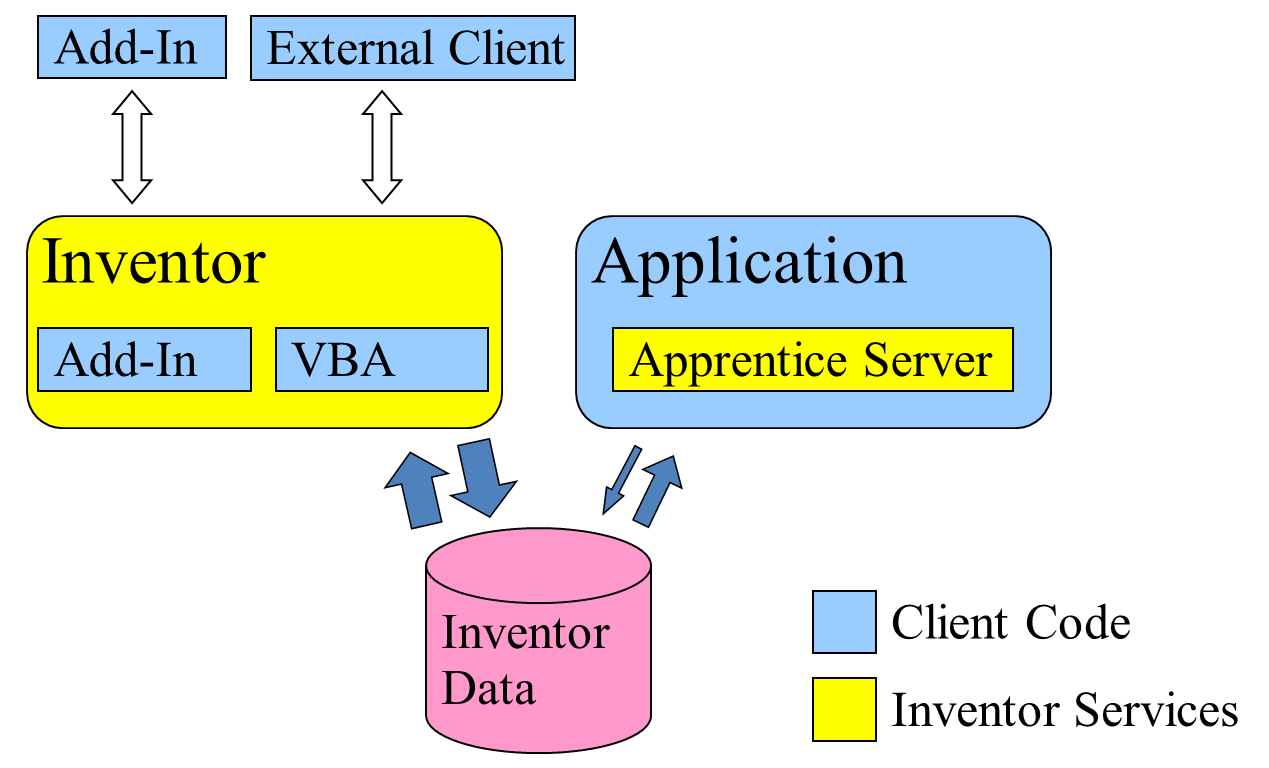
\includegraphics[width=0.9\linewidth]{../Common/images/InventorAPI.png}
\vspace{2mm}
\textbf{Decision} : Out-of-Process/External VB.Net application 
\end{frame}

%-------------------------------------------------------------------------------------

\begin{frame}{Sample Program Screen Shot}

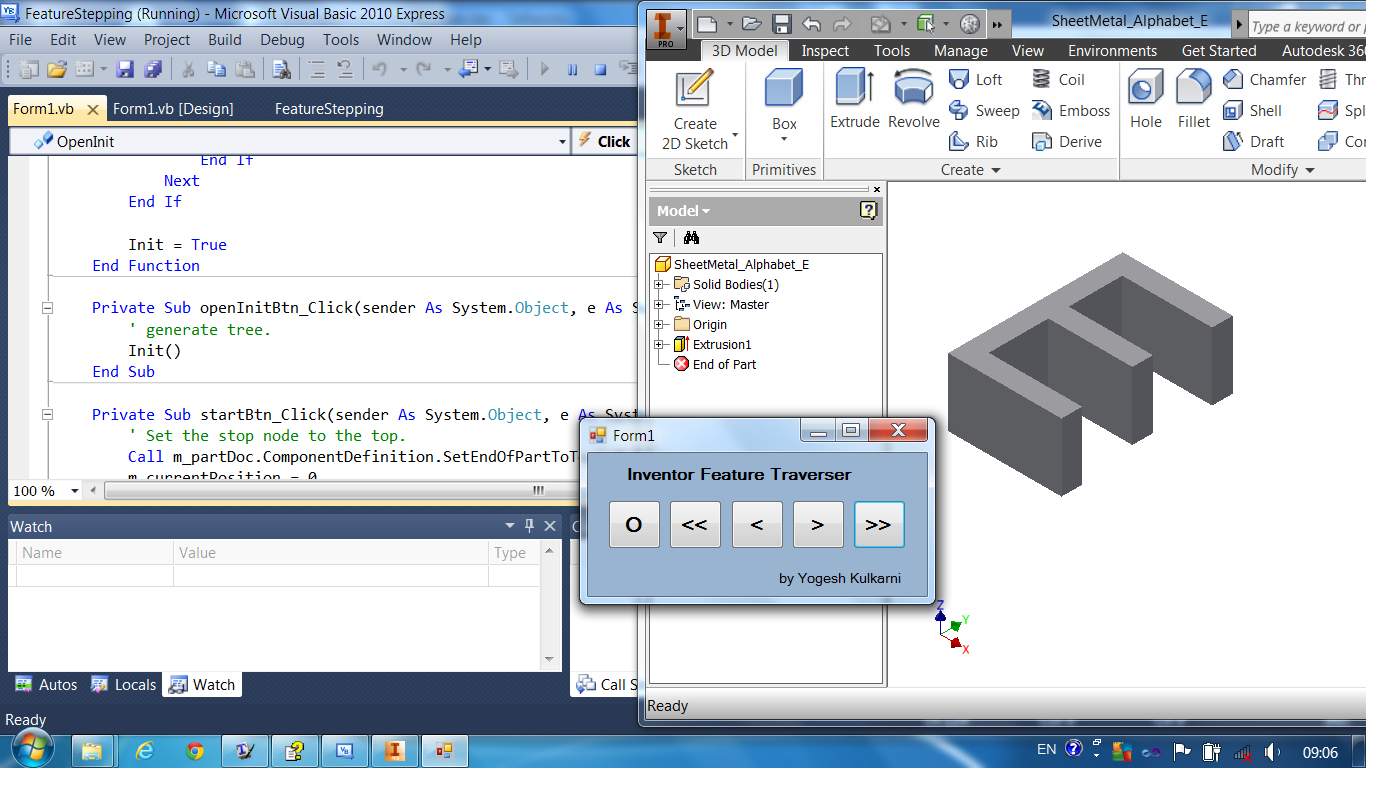
\includegraphics[width=0.9\linewidth]{../Common/images/ImplSampleProgram.png}
\end{frame}

%-------------------------------------------------------------------------------------
